\documentclass[a4paper,10pt]{article}
%\usepackage[latin1]{inputenc} % Paquetes de idioma
\usepackage[utf8]{inputenc} % Paquetes de idioma (Este encoding toma acentos :) )
\usepackage[spanish]{babel} % Paquetes de idioma
\usepackage{graphicx} % Paquete para ingresar gráficos
\usepackage{grffile}
\usepackage{hyperref}
\usepackage{fancybox}
\usepackage{amsmath}
\usepackage{amsfonts}
\usepackage{listings}
\usepackage{float}
% Paquetes de macros de Circuitos
%\usepackage{pstricks}
\usepackage{tikz}

% Encabezado y Pié de página
\usepackage{fancyhdr} % Paquete para encabezados y pie de página
\pagestyle{fancy} % Sin esta línea no se imprimiría el encabezado en todas las páginas

\fancyhf{} %  Borra el encabezado anterior (Por defecto escribe el títutlo de la sección en la que se encuentra la hoja
\setlength{\headheight}{22.55pt}
\fancyhead[L]{
	{\textsf{Facultad de Ingenier\'ia $-$ Universidad de Buenos Aires \\ 66.44 Instrumentos Electrónicos}}
}
%\addtocounter{page}{5}
\fancyhead[R]{\thepage}

\renewcommand{\footrulewidth}{0.4pt} % Ajusta el tamaño de las líneas separadoras en el pié de página
\renewcommand{\headrulewidth}{0.4pt} % Ajusta el tamaño de las líneas separadoras en el encabezado

\fancyfoot[L]{
	{\textsf{Trabajo Pr\'actico N$^{\circ}4$}: Mediciones de impedancias} \\
	{\textsf{Integrantes: Eduardo Sanchez, Francisco Soler}}
	}
		

% Carátula del Trabajo
\title{ \author{} % Lo pongo para que el warning no moleste :p
\setlength{\unitlength}{1cm} %  Especifica la unidad de trabajo
\thispagestyle{empty}

\begin{picture}(18,0)
\put(0,0){
\includegraphics[width=1.5cm, height=3cm]{Logo1.png}}

\put(10.5,0){
\includegraphics[width=3cm, height=3cm]{Logo2.png}}

\end{picture}
\\[1.5cm]
\begin{center}
	\textbf{{\Huge Facultad de Ingenier\'ia \\ Universidad de Buenos Aires}}\\[2cm]
	{66.44 Instrumentos Electrónicos}\\[0.5cm]
	{Trabajo Pr\'actico N$^{\circ}3$: Mediciones de impedancias}\\[2.5cm]
\end{center}

\begin{flushleft}
	\textbf{Integrantes:} \\[1cm]

	\begin{tabular}{|c|c|c|}
		\hline
		\textbf{\normalsize Padr\'on} & \textbf{\normalsize Nombre} & \textbf{\normalsize Email} \\
		\hline
		\normalsize 92903 & \normalsize Sanchez, Eduardo Hugo & \normalsize hugo\_044@hotmail.com \\
		\hline
		\normalsize 91227 & \normalsize Soler, Jos\'e Francisco & \normalsize francisco.\_tw@hotmail.com \\
		\hline
		\normalsize xxx & \normalsize Wawrynczak, Claudio  & \normalsize claudiozak@gmail.com \\
		\hline
	\end{tabular}
\end{flushleft}
\date{} % Hace que no se imprima la fecha en la cual se compilo el .tex
 }

\begin{document}
	\maketitle % Hace que el título anterior sea el principal del documento
	\newpage

	\tableofcontents % Esta línea genera un indice a partir de las secciones y subsecciones creadas en el documento
	\newpage


	\section{Objetivo}
	
	\indent	El objetivo del presente trabajo práctico es determinar el comportamiento y fiabilidad de 3 tipos de puntas de medición, de tensión con alta/baja impedancia de entrada, y de corriente.
	
	\newpage
	\section{Desarrollo}
		\indent Para llevar a cabo las mediciones, se utilizan los siguientes instrumentos:
		\begin{itemize}
			\item Un generador de señales con la capacidad de realizar un barrido en frecuencias.
			\item Un osciloscopio con la capacidad de cambiar a alta o baja su impedancia de entrada.
			\item Las puntas de prueba.
			\item Un cable que interconecta el generador con el osciloscopio, el cual, se comporta como una línea de transmisión.
		\end{itemize}
				 
		\subsection{Punta de prueba de alta impedancia}
		\subsection{Punta de prueba de baja impedancia}
		\subsection{Punta de prueba de corriente}
		
		
	\section{Conclusi\'on}
		\indent Es importante conocer bien las características de las puntas a utilizar, como del osciloscopio y del circuito a medir, para poder determinar si la medición se la puede tomar como válida.
		\indent Como conclusiones se puede decir que las puntas de alta impedancias poseen un rango dinámico mucho mayor que las de baja impedancia. Las puntas de baja impedancia, al tener un BW infinito, en áltas frecuencias terminan teniendo una impedancia de entrada mayor que las de alta impedancia.
		\indent Otro tema a tener en cuenta es que no siempre el ancho de banda es el calculado, dado que en ciertas circunstancias la parte plana de la señal no es lo suficinetemente plana y puede llegar a caer 3db en una zona (dado que la atenuación de la punta depende de la frecuencia) menor al punto donde se encuentra el polo dominante.
		
		
		
		\indent Para este escenario, al cable utilizado se lo tuvo que romper para que entre dentro de las puntas de corriente, esto logra un cambio de la impedancia en el mismo por la disminución de la sección (generando así reflexiones y distorsiones en la señal).
		
		\indent IPsec (Internet Protocol security) es un conjunto de protocolos cuya función es asegurar las comunicaciones sobre el Protocolo de Internet (IP) autenticando y/o cifrando cada paquete IP en un flujo de datos. IPsec también incluye protocolos para el establecimiento de claves de cifrado.\\
	\indent Los protocolos de IPsec actúan en la capa de red (capa 3). Otros protocolos de seguridad para Internet, como SSL, TLS y SSH operan de la capa de transporte (capas OSI 4 a 7) hacia arriba. Esto hace que IPsec sea más flexible, ya que puede ser utilizado para proteger protocolos de la capa 4, incluyendo TCP y UDP. Otra ventaja es que para que una aplicación pueda usar IPsec no hay que hacer ningún cambio, mientras que para usar SSL y otros protocolos de niveles superiores, las aplicaciones tienen que modificar su código. \\
	\indent IPsec está implementado por un conjunto de protocolos criptográficos para:
	
	\begin{itemize}
		\item Asegurar el flujo de paquetes.
		\item Garantizar la autenticación mutua.
		\item Establecer parámetros criptográficos.
	\end{itemize}		

	\indent La arquitectura de seguridad IP utiliza el concepto de asociación de seguridad (SA) como base para construir funciones de seguridad en IP. Una asociación de seguridad es simplemente el paquete de algoritmos y parámetros (tales como las claves) que se está usando para cifrar y autenticar un flujo particular en una dirección. Por lo tanto, en el tráfico normal bidireccional, los flujos son asegurados por un par de asociaciones de seguridad. La decisión final de los algoritmos de cifrado y autenticación (de una lista definida) le corresponde al administrador de IPsec. \\
	\indent Para decidir qué protección se va a proporcionar a un paquete saliente, IPsec utiliza el índice de parámetro de seguridad (SPI), un índice a la base de datos de asociaciones de seguridad (SADB), junto con la dirección de destino de la cabecera del paquete, que juntos identifican de forma única una asociación de seguridad para dicho paquete. Para un paquete entrante se realiza un procedimiento similar; en este caso IPsec utiliza las claves de verificación y descifrado de la base de datos de las asociaciones de seguridad. \\
	\indent En el caso de multicast, se proporciona una asociación de seguridad al grupo, y se duplica para todos los receptores autorizados del grupo. Puede haber más de una asociación de seguridad para un grupo, utilizando diferentes SPIs, y por ello permitiendo múltiples niveles y conjuntos de seguridad dentro de un grupo. De hecho, cada remitente puede tener múltiples asociaciones de seguridad, permitiendo autenticación, ya que un receptor sólo puede saber que alguien que conoce las claves ha enviado los datos. Hay que observar que el estándar pertinente no describe cómo se elige y duplica la asociación a través del grupo; se asume que un interesado responsable habrá hecho la elección.
	
	
	
	
		\subsection{Modos de funcionamiento}
			\subsubsection{Modo transporte}
	\indent En modo transporte, sólo la carga útil (los datos que se transfieren) del paquete IP es cifrada y/o autenticada. El enrutamiento permanece intacto, ya que no se modifica ni se cifra la cabecera IP; sin embargo, cuando se utiliza la cabecera de autenticación (AH), las direcciones IP no pueden ser traducidas, ya que eso invalidaría el hash. Las capas de transporte y aplicación están siempre aseguradas por un hash, de forma que no pueden ser modificadas de ninguna manera (por ejemplo traduciendo los números de puerto TCP y UDP). El modo transporte se utiliza para comunicaciones ordenador a ordenador. \\
	\indent Una forma de encapsular mensajes IPsec para atravesar NAT ha sido definido por RFCs que describen el mecanismo de NAT-T. \\
	\indent El propósito de este modo es establecer una comunicación segura punto a punto, entre dos hosts y sobre un canal inseguro. La imagen \ref{img001} ilustra esto:
	
	\begin{figure}[!htb]
		\centering
		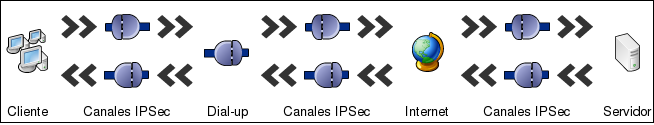
\includegraphics[width=11cm]{Imagenes/ipSecModoTransporte.png}
		\caption{Esquemático de IPSec en modo transporte} \label{img001}
	\end{figure}


			\subsubsection{Modo t\'unel}
	
	\indent En el modo túnel, todo el paquete IP (datos más cabeceras del mensaje) es cifrado y/o autenticado. Debe ser entonces encapsulado en un nuevo paquete IP para que funcione el enrutamiento. El modo túnel se utiliza para comunicaciones red a red (túneles seguros entre routers, ejemplo, para VPNs) o comunicaciones ordenador a red u ordenador a ordenador sobre Internet. El propósito de este modo es establecer una comunicación segura entre dos redes remotas sobre un canal inseguro. La imagen \ref{img002} ilustra esto:
			
	\begin{figure}[!htb]
		\centering
		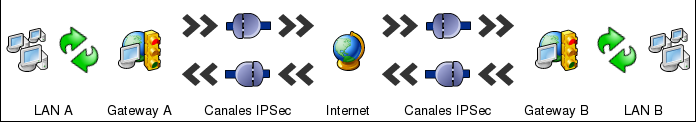
\includegraphics[width=11cm]{Imagenes/ipSecModoTunel.png}
		\caption{Esquemático de IPSec en modo t\'unel} \label{img002}
	\end{figure}

		\subsection{Protocolo AH}
	\indent AH está dirigido a garantizar integridad sin conexión y autenticación de los datos de origen de los datagramas IP. Para ello, calcula un Hash Message Authentication Code (HMAC) a través de algún algoritmo hash operando sobre una clave secreta, el contenido del paquete IP y las partes inmutables del datagrama. Este proceso restringe la posibilidad de emplear NAT, que puede ser implementada con NAT transversal. Por otro lado, AH puede proteger opcionalmente contra ataques de repetición utilizando la técnica de ventana deslizante y descartando paquetes viejos. AH protege la carga útil IP y todos los campos de la cabecera de un datagrama IP excepto los campos mutantes, es decir, aquellos que pueden ser alterados en el tránsito. En IPv4, los campos de la cabecera IP mutantes (y por lo tanto no autenticados) incluyen TOS, Flags, Offset de fragmentos, TTL y suma de verificación de la cabecera. AH opera directamente por encima de IP, utilizando el protocolo IP número 51. Un cabecera AH mide 32 bits, la figura \ref{img003} muestra un diagrama de cómo se organizan:
	
	\begin{itemize}
		\item next hdr: Identifica cuál es el siguiente protocolo, es decir, cual es el protocolo que será autentificado, cuál es el payload.
		\item AH len: El tamaño del paquete AH.
		\item RESERVED: Reservado para futuras aplicaciones. Debe ser igual a 0.
		\item Security parameters index (SPI): Indica los parametros de seguridad, que en combinación con los parámetros IP, identifican la asociación de seguridad del paquete.
		\item Sequence Number: Es un número creciente usado para prevenir ataques por repetición. El número está incluido en los datos encriptados, así que cualquier alteración será detectada.
		\item Authentication Data: Contiene el valor de identificación de integridad. Puede contener relleno. Se calcula sobre el paquete entero, incluidas la mayoría de las cabeceras. El que recibe calcula otra vez el hash, y si este no coincide, el paquete se descarta.
	\end{itemize}		
	
	\begin{figure}[!htb]
		\centering
		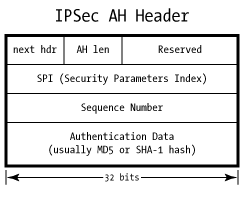
\includegraphics[width=7cm]{Imagenes/cabeceraIPSecAH.png}
		\caption{Cabecera IPSec AH} \label{img003}
	\end{figure}
	
	
	
	\newpage
		\subsection{Protocolo ESP}
	\indent Añadir encriptación hace que ESP sea un poco más complicado que AH: ESP incluye cabecera y campos para dar soporte a la encriptacion y a una autentificación opcional. Además, provee los modos de transporte y túnel. \\
	\indent Los sistemas de encriptaci\'on m\'as utilizados son DES, triple-DES, AES o Blowfish para asegurar la carga útil de “ojos indiscretos”. El algoritmo usado para una conexión en particular es definido por la Security Association (SA), y esta SA incluye no sólo la el algoritmo, también la llave usada. \\
	\indent A diferencia de AH, que da una pequeña cabecera antes de la carga útil, ESP rodea la carga útil con su protección. Los parámetros de seguridad Index y Sequence Number tienen el mismo propósito que en AH, pero agrega  relleno al final del paquete antes del campo “siguiente campo” y el opcional “Authentication data”. \\
	\indent Es posible usar ESP sin ninguna encriptación (usar el algoritmo NULL), sin embargo estructura del paquete es de la misma forma y no brinda ninguna confidencialidad a los datos que estamos transmitiendo. \\
	\indent El relleno sirve para poder usar algoritmos de encriptación orientados a bloques, dado que se tiene que crear una carga a encriptar que tenga un tamaño múltiplo de su tamaño de bloque. El tamaño del relleno viene dado por el campo pad len. El campo next hdr brinda el tipo (IP, TCP, UDP, etc) de la carga útil, aunque esto sea usado como un punto para volver hacia atras en el paquete para ver que hay en el AH. \\
	\indent Además de la encriptación, ESP puede proveer autentificación con la misma HMAC de AH. A diferencia de AH, esta autentifica sólo la cabecera ESP y la carca útil encriptada, no todo el paquete IP. Esto no hace que la seguridad de la autentificación más débil, pero nos da algunos beneficios importantes. \\
	\indent Cuando un forastero examina un paquete IP que contiene datos ESP, es prácticamente imposible adivinar que es lo que tiene dentro, excepto por los datos encontrados en la cabecera IP (siendo interesantes las direcciones IP de origen y destino). El atacante va a saber casi seguro que son datos ESP (está en la cabecera que son datos ESP), pero no va a saber de que tipo es la carga útil. El gr\'afico \ref{img004} muestra las cabeceras del protocolo.\\

	\begin{figure}[!htb]
		\centering
		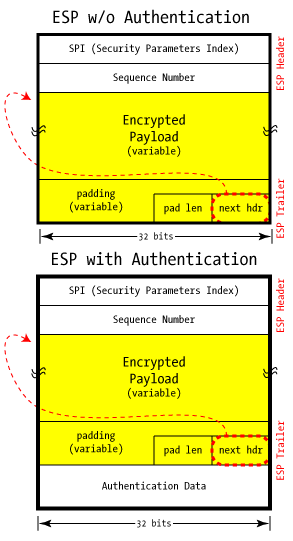
\includegraphics[height=10cm]{Imagenes/protocoloEsp.png}
		\caption{Cabeceras IPSec ESP} \label{img004}
	\end{figure}	

	

	\newpage
	\section{Desarrollo}
		\subsection{Configuración de las máquinas virtuales}

	\indent Para realizar la práctica se levantarán cuatro máquinas virtuales con el sistema VirtualBox. 
	\indent Las Vm fueron conectadas de la forma como muestra la figura \ref{img005} y, como se mencionó previamente cada una cumple la funcionalidad de cada componente de la red.

	
	\begin{figure}[!htb]
		\centering
		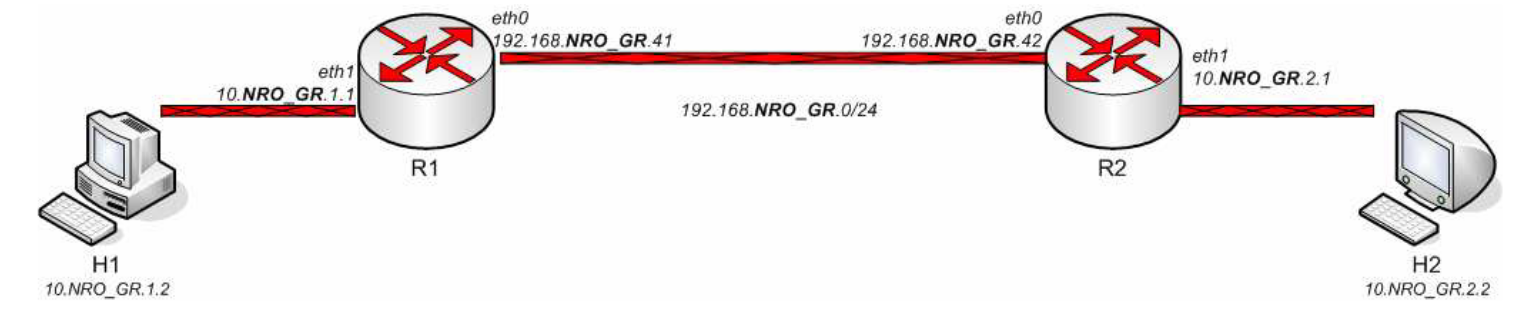
\includegraphics[width=11cm]{Imagenes/red.png}
		\caption{red de VMs} \label{img005}
	\end{figure}
	
		\subsection{Configuración de adaptadores}
	\indent A continuaci\'on se configurar\'an los adaptadores de red de cada VM para poder armar la red propuesta.	
			\subsubsection{Configuración del adaptador de red de H1}	
	\begin{figure}[!htb]
		\centering
		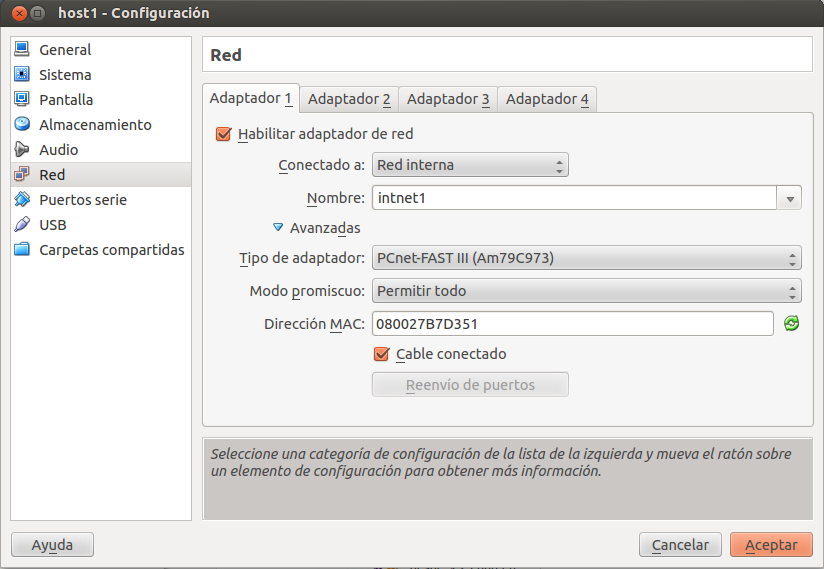
\includegraphics[width=11cm]{Imagenes/Host1ConfigAdaptador.png}
		\caption{Configuración del adaptador de red de H1} \label{img006}
	\end{figure}

			\subsubsection{Configuración del adaptador de red de H2}	
	\begin{figure}[!htb]
		\centering
		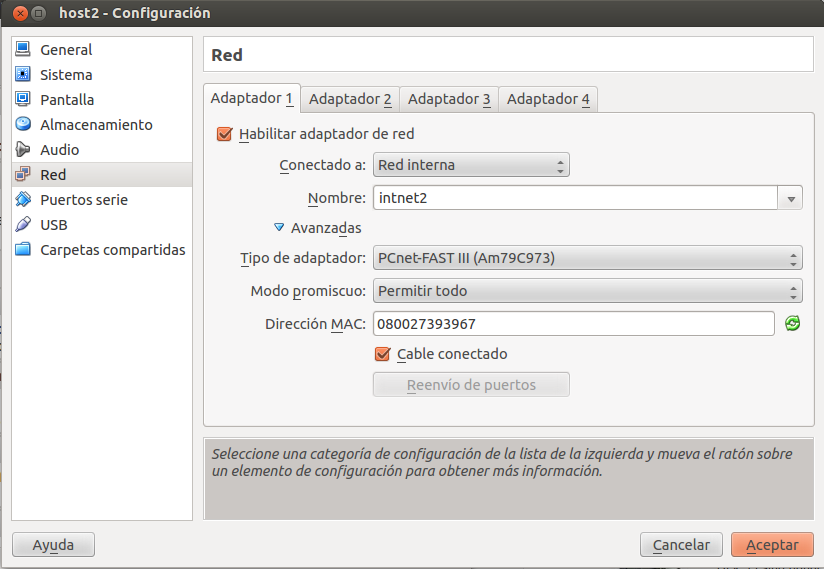
\includegraphics[width=11cm]{Imagenes/Host2ConfigAdaptador1.png}
		\caption{Configuración del adaptador de red de H2} \label{img007}
	\end{figure}

			\subsubsection{Configuración del adaptador de red de R1}	
	\begin{figure}[!htb]
		\centering
		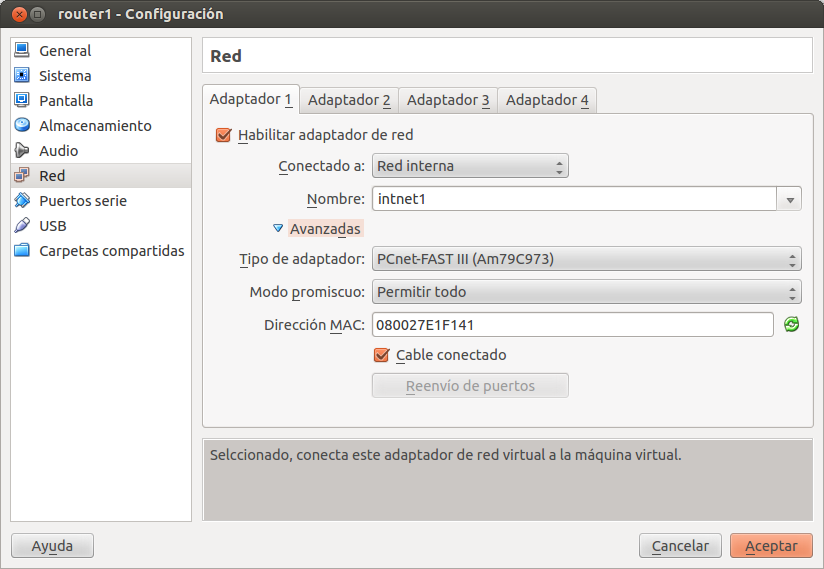
\includegraphics[width=11cm]{Imagenes/router1ConfigAdaptador1.png}
		\caption{Configuración del adaptador 1 de red de R1} \label{img008}
	\end{figure}
	\begin{figure}[!htb]
		\centering
		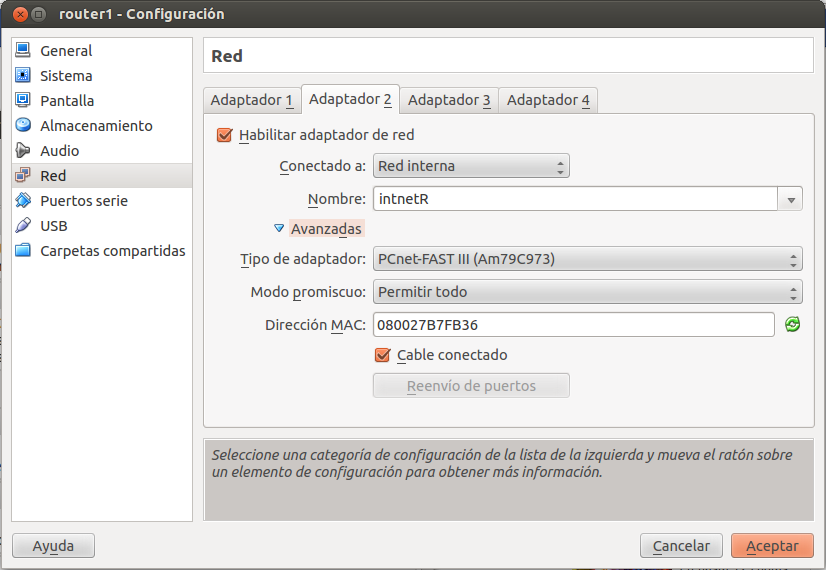
\includegraphics[width=11cm]{Imagenes/Router1ConfigAdaptador2.png}
		\caption{Configuración del adaptador 2 de red de R1} \label{img009}
	\end{figure}
	
			\subsubsection{Configuración del adaptador de red de R2}	
	\begin{figure}[!htb]
		\centering
		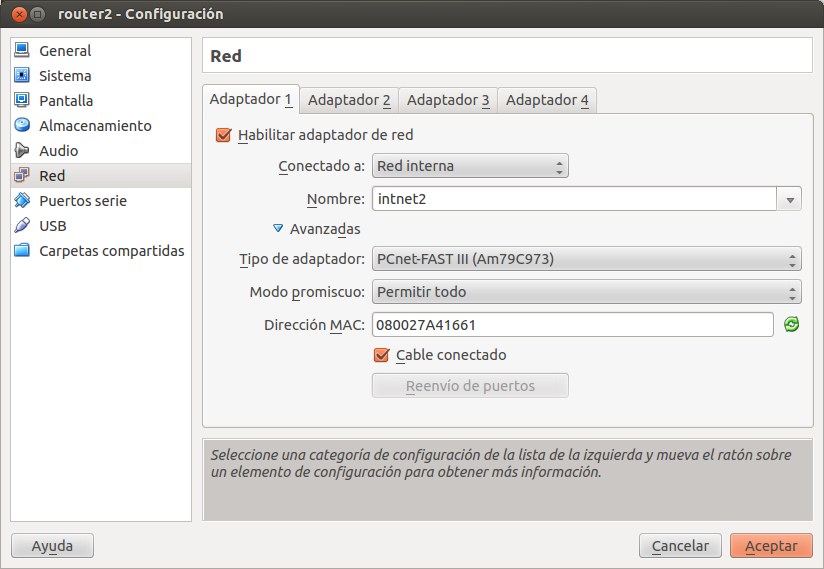
\includegraphics[width=11cm]{Imagenes/Router2ConfigAdaptador1.png}
		\caption{Configuración del adaptador 1 de red de R2} \label{img010}
	\end{figure}	
	\begin{figure}[!htb]
		\centering
		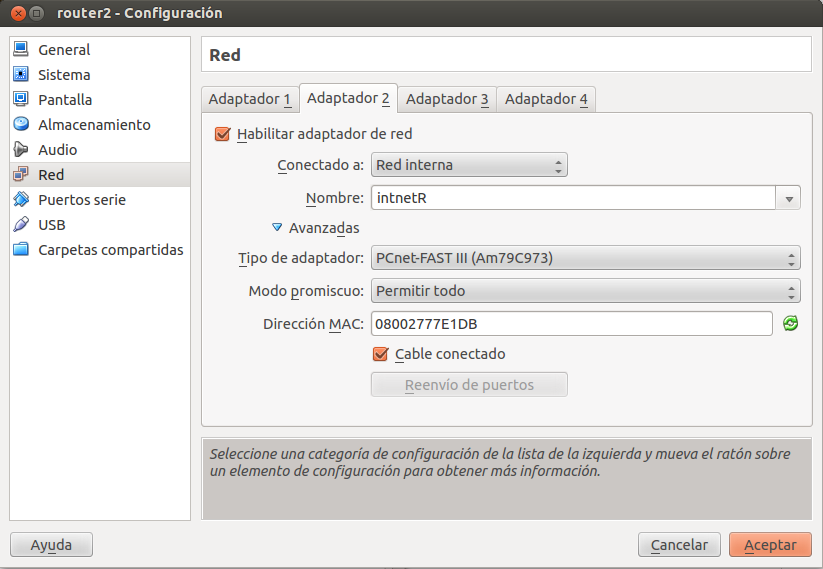
\includegraphics[width=11cm]{Imagenes/Router2ConfigAdaptador2.png}
		\caption{Configuración del adaptador 2 de red de R2} \label{img011}
	\end{figure}		
		
		\subsection{Configuraci\'on de redes y VMs}	
	\indent A continuaci\'on se configurar\'an las redes as\'i como los routers y hosts. Primero se debe elegir en que redes se va a trabajar, para ello hay que determinar en el archivo /crypto/conf/config.sh el número de grupo. En la presente prueba se utilizó el número 1. A su vez hay que serciorarse que el tipo de túnel sea ESP-RSA.
	\indent Estos pasos deben realizarse para cada VM. Se mostrará una sola imagen a modo ilustrativo(ver figuras números \ref{img012} y \ref{img013}).
	
	\begin{figure}[!htb]
		\centering
		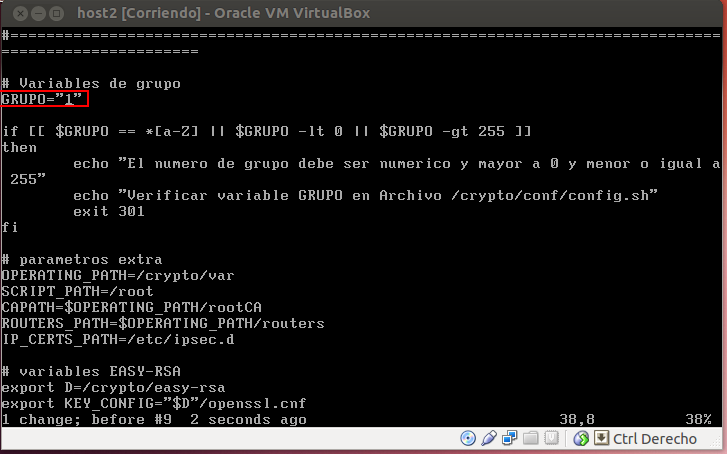
\includegraphics[width=11cm]{Imagenes/chequeoNombreGrupo.png}
		\caption{chequeo el número del grupo} \label{img012}
	\end{figure}	
	\begin{figure}[!htb]
		\centering
		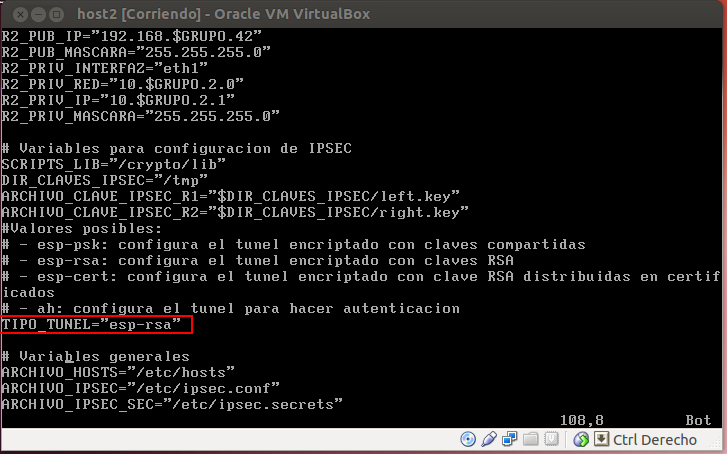
\includegraphics[width=11cm]{Imagenes/chequeoTipoTunel.png}
		\caption{Chequeo el tipo de túnel} \label{img013}
	\end{figure}	

			\subsubsection{Configuraci\'on de R1}
	\begin{figure}[H]
		\centering
		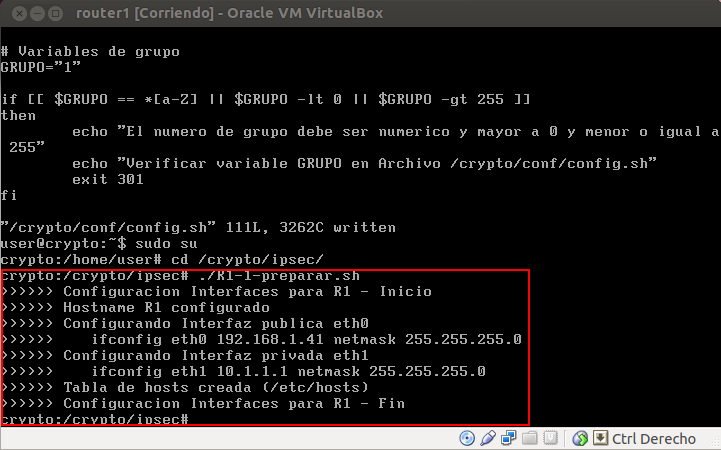
\includegraphics[width=11cm]{Imagenes/prepararR1.png}
		\caption{Configuraci\'on de las interfaces de R1} \label{img014}
	\end{figure}	

			\subsubsection{Configuraci\'on de R2}
	\begin{figure}[H]
		\centering
		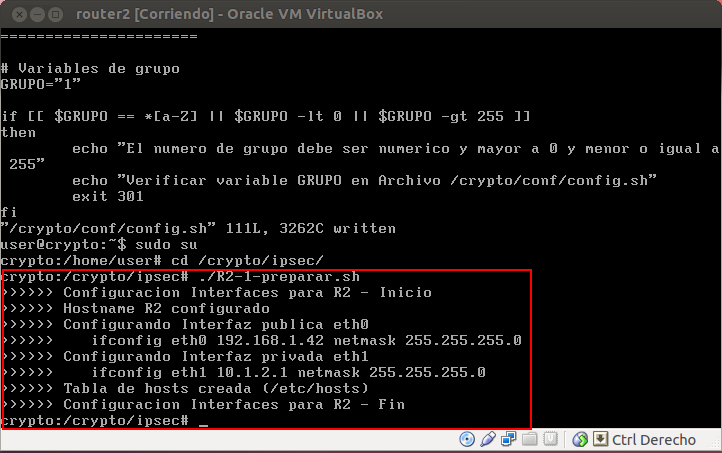
\includegraphics[width=11cm]{Imagenes/prepararR2.png}
		\caption{Configuraci\'on de las interfaces de R2} \label{img015}
	\end{figure}	

			\subsubsection{Configuraci\'on de H1}
	\begin{figure}[H]
		\centering
		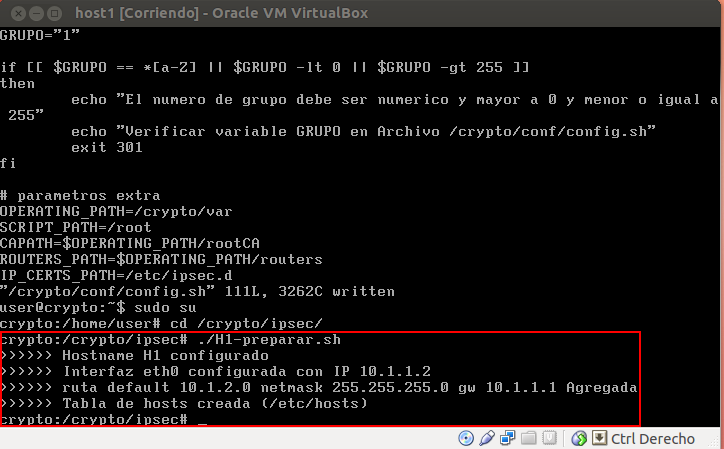
\includegraphics[width=11cm]{Imagenes/prepararH1.png}
		\caption{Configuraci\'on de las interfaces de H1} \label{img016}
	\end{figure}	

			\subsubsection{Configuraci\'on de H2}
	\begin{figure}[H]
		\centering
		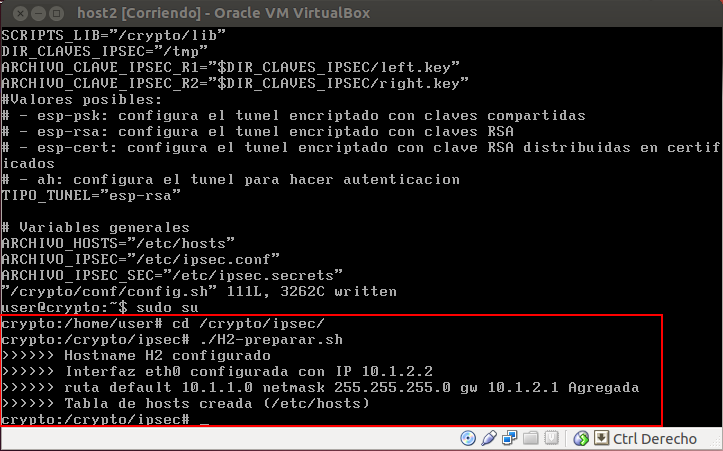
\includegraphics[width=11cm]{Imagenes/prepararH2.png}
		\caption{Configuraci\'on de las interfaces de H2} \label{img017}
	\end{figure}	
	
		\subsection{Verificación de la comunicación}
	\indent Para verificar la comunicaci\'on se realizar\'an pings entre los siguientes pares H1 a R1, R1 a R2 y H2 a R2. Ver figuras \ref{img018}, \ref{img019} y \ref{img020}
	\begin{figure}[H]
		\centering
		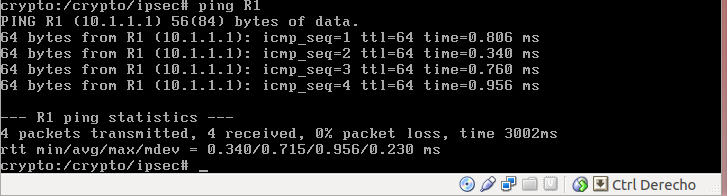
\includegraphics[width=11cm]{Imagenes/pingH1aR1.png}
		\caption{Pings de H1 a R1} \label{img018}
	\end{figure}	
	\begin{figure}[H]
		\centering
		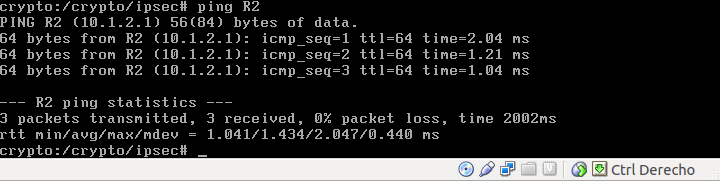
\includegraphics[width=11cm]{Imagenes/pingH2aR2.png}
		\caption{Pings de H2 a R2} \label{img019}
	\end{figure}	
	\begin{figure}[H]
		\centering
		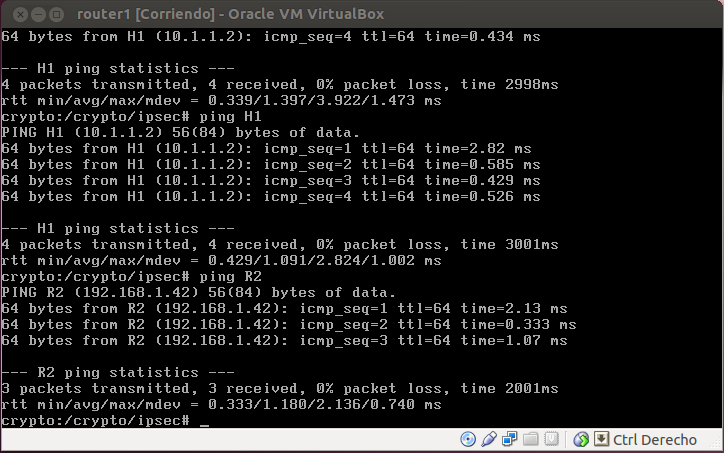
\includegraphics[width=11cm]{Imagenes/pingR1aR2.png}
		\caption{Pings de H1 a R2} \label{img020}
	\end{figure}	
	
	\indent Se puede observar que no se perdieron los pings, por lo tanto la red está bien configurada.
	
		\subsection{Configuracion t\'unel IPSEC}
	\indent A continuaci\'on se configurar\'a el t\'unel IPSec entre R1 y R2.
			
			\subsubsection{Generación de claves IPSEC}
	\begin{figure}[H]
		\centering
		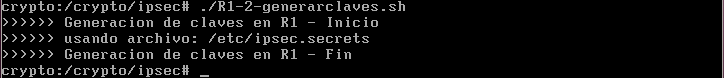
\includegraphics[width=11cm]{Imagenes/generarClaveR1.png}
		\caption{Generar Claves de IPSec en R1}
	\end{figure}	
	\begin{figure}[H]
		\centering
		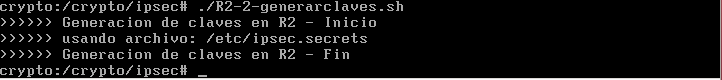
\includegraphics[width=11cm]{Imagenes/generarClaveR2.png}
		\caption{Generar Claves de IPSec en R2}
	\end{figure}			
			
			\subsubsection{Obtención de la claves IPSEC}
	\begin{figure}[H]
		\centering
		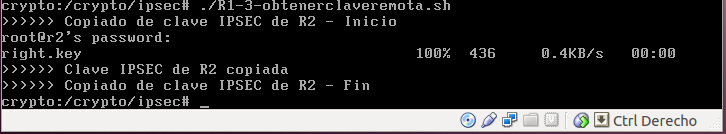
\includegraphics[width=11cm]{Imagenes/obtencionClaveIPsecR1.png}
		\caption{Obtener Claves de IPSec en R1}
	\end{figure}	
	\begin{figure}[H]
		\centering
		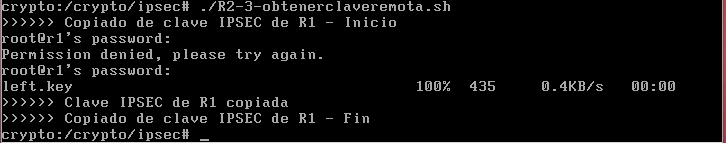
\includegraphics[width=11cm]{Imagenes/obtencionClaveIPsecR2.png}
		\caption{Obtener Claves de IPSec en R2}
	\end{figure}		
	
			\subsubsection{Configuración de IPSEC}	
	\begin{figure}[H]
		\centering
		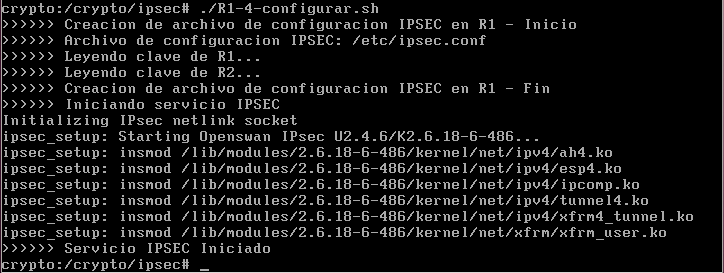
\includegraphics[width=11cm]{Imagenes/configurarIPsecR1.png}
		\caption{Configuración de IPSec en R1}
	\end{figure}	
	\begin{figure}[H]
		\centering
		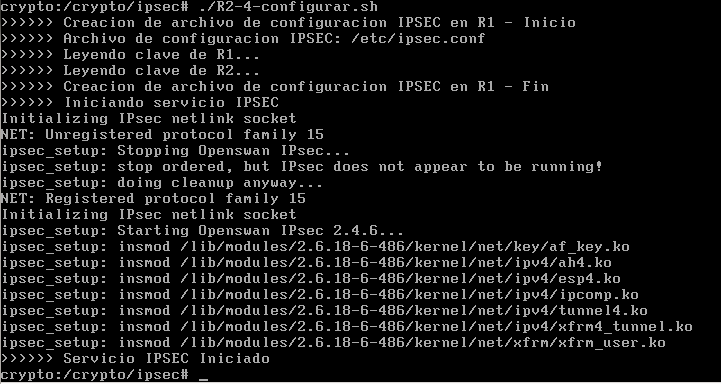
\includegraphics[width=11cm]{Imagenes/configurarIPsecR2.png}
		\caption{Configuración de IPSec en R2}
	\end{figure}	
	
			\subsubsection{Inicialización del enlace IPSEC}	
	\begin{figure}[H]
		\centering
		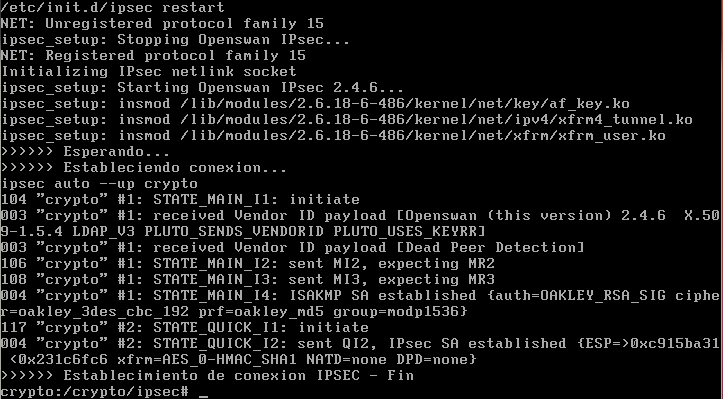
\includegraphics[width=11cm]{Imagenes/inicializarEnlaceIPsec.png}
		\caption{Inicializaci\'on del enlace IPSec}
	\end{figure}	
	
		\subsection{Verificaci\'on del t\'unel}	
			Para la verificación del túnel primero se observa que estén las tablas de routeo correspondientes en ambos routers y se realizarán pings de H1 a H2 y viceversa para determinar que se pueden comunicar entre sí. Ver gráficos \ref{img021}, \ref{img022}, \ref{img023} y \ref{img024}
			
	\begin{figure}[H]
		\centering
		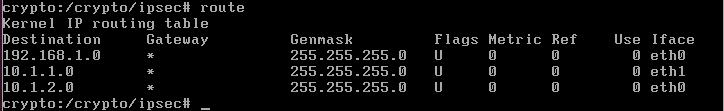
\includegraphics[width=11cm]{Imagenes/tablaRouteoR1.png}
		\caption{Tabla del router R1}\label{img021}
	\end{figure}	
	\begin{figure}[H]
		\centering
		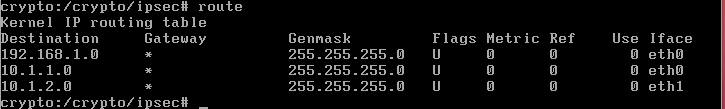
\includegraphics[width=11cm]{Imagenes/tablaRouteoR2.png}
		\caption{Tabla del router R2}\label{img022}
	\end{figure}	
	\begin{figure}[H]
		\centering
		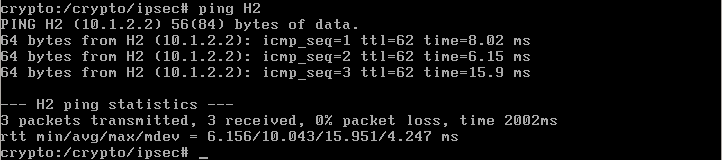
\includegraphics[width=11cm]{Imagenes/pingH1H2ConIPsec.png}
		\caption{pings de H1 a H2 con IPSec}\label{img023}
	\end{figure}	
	\begin{figure}[H]
		\centering
		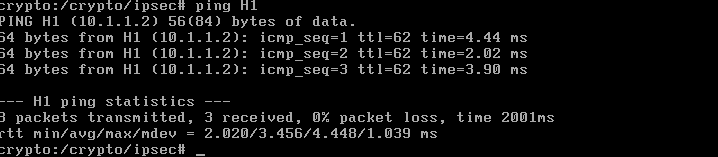
\includegraphics[width=11cm]{Imagenes/pingH2H1ConIPsec.png}
		\caption{pings de H2 a H1 con IPSec}\label{img024}
	\end{figure}	
	
		\subsection{Análisis del tráfico}
	\indent A continuación se correrá el wireshark sobre la interfaz eth0, y se observará que tipo de tráfico hay.
	
	\begin{figure}[H]
		\centering
		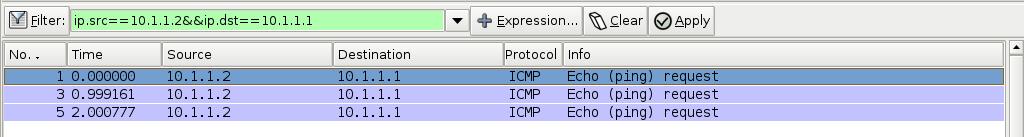
\includegraphics[width=11cm]{Imagenes/pingH1R1.png}
		\caption{tráfico en la red entre H1 y R1}
	\end{figure}	

	
	\indent Se puede observar solo los paquetes ICMP enviados por el host 1. No se observan paquetes ESP ya que esa comunicación no está todavía en el túnel IPSec. \\
	\indent Ahora se observará el tráfico entre R1 y R2 al hacer un ping tanto de H2-H1, ver figura \ref{img025}

	\begin{figure}[H]
		\centering
		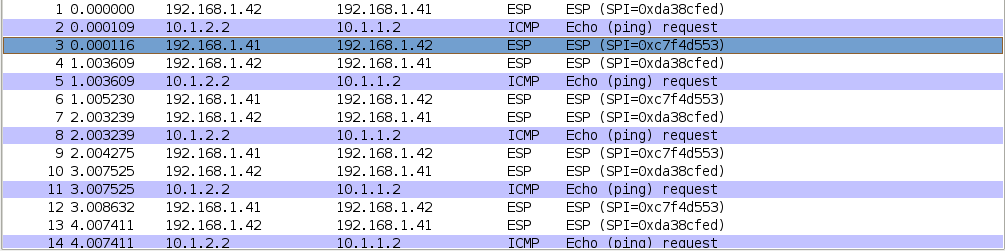
\includegraphics[width=11cm]{Imagenes/paquetesESP.png}
		\caption{tr\'afico dentro del t\'unel}\label{img025}
	\end{figure}	
	
	\indent Como se puede observar, los paquetes entre los routers (192.168.1.41 a 192.168.1.42 y viceversa) son paquetes ESP propios del túnel. Tambien se ve como el túnel encripta con los paquetes ESP los request de los paquetes ICMP. \\
	\indent Analizando algún paquete ESP podemos verificar por ejemplo, como el datagrama IP tiene el valor 50 (0x32 en hexadecimal) en el campo del protocolo (ver figura \ref{img026}). A su vez, se observa que está en modo túnel el enlace ya que los destinos y orígenes están en encapsulados dentro del datagrama y en estas direcciones. En el exterior del datagrama IP figuran las IPs de la red que conecta los routers (ver figura \ref{img027}).
	
	\begin{figure}[H]
		\centering
		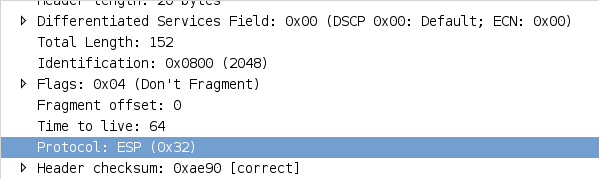
\includegraphics[width=11cm]{Imagenes/protocoloESP.png}
		\caption{protocolo utilizado por el túnel IPSec}\label{img026}
	\end{figure}	
	\begin{figure}[H]
		\centering
		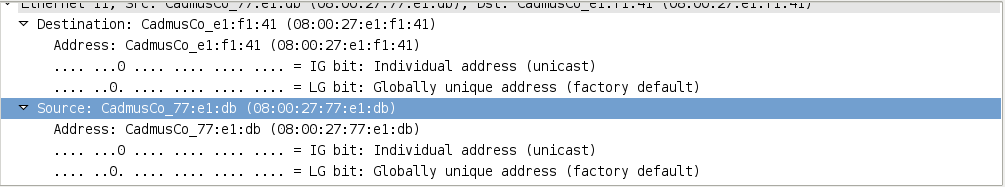
\includegraphics[width=11cm]{Imagenes/DestOrigenEncriptados.png}
		\caption{Destinos y origenes encriptados}\label{img027}
	\end{figure}	
	
	\indent Para establecer el enlace se ejecutan dos fases, las cuales son el Main Mode (Identity Protection) y el Quick Mode. \\
	\indent El Main Mode es el encargado de generar un canal seguro en el cual se puedan intercambiar los datos necesarios de la segunda fase. El intercambio de las claves se realiza utilizando Diffie-Hellman y luego se autentica a cada una de las partes. En la fase Quick Mode es en donde se produce la negociación de las IPSec SA’s para poder generar el túnel IPSec. Se actualiza la información utilizada para encriptar, así como también se actualizan de forma periodica las SA’s. El gráfico número \ref{img028} muestra la comunicación.
	
	\begin{figure}[!hfe]
		\centering
		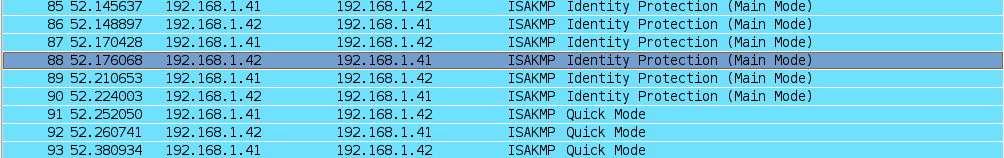
\includegraphics[width=11cm]{Imagenes/establecimientoConexion.png}
		\caption{comunicación entre routers al establecer conexión}\label{img028}
	\end{figure}	

		\subsection{Desencriptación del tráfico}
	\indent Para desencriptar el tráfico se ejecuta el comando setkey -D. \\		\indent Se agregan los datos obtenidos (mostrados en la figura \ref{img029}) a la configuración del WireShark tal como está indicado en el enunciado del trabajo práctico. \\
	\indent	La figura \ref{img030} muestra como el paquete de ICMP esta desencriptado. Se pueden apreciar las direcciones origen y destino dentro del paquete tanto del enlace R1-R2 como de los hosts H1-H2.  \\
	\indent Al bajar el tunel y volver a levantarlo las claves se pierden y no es posible desencriptar el tráfico sin actualizar las mismas en el programa. Ver gráfico \ref{img031}
 
		
	\begin{figure}[H]
		\centering
		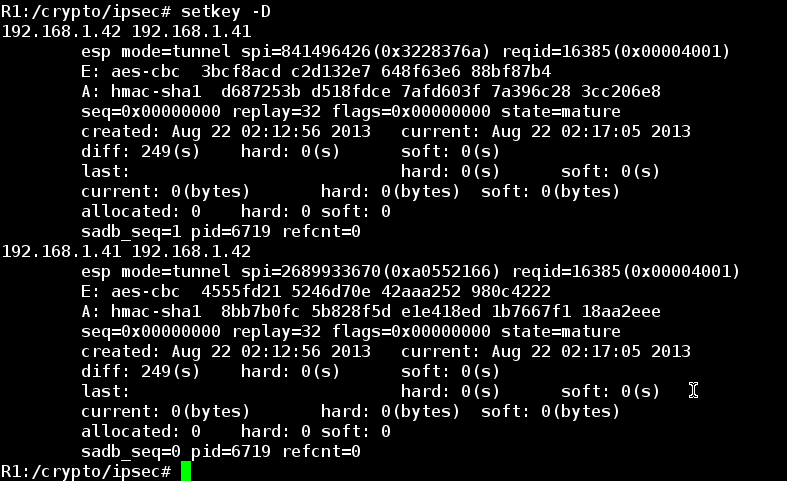
\includegraphics[width=11cm]{Imagenes/setKey.png}
		\caption{Desencriptando el tr\'afico}\label{img029}
	\end{figure}	
	\begin{figure}[H]
		\centering
		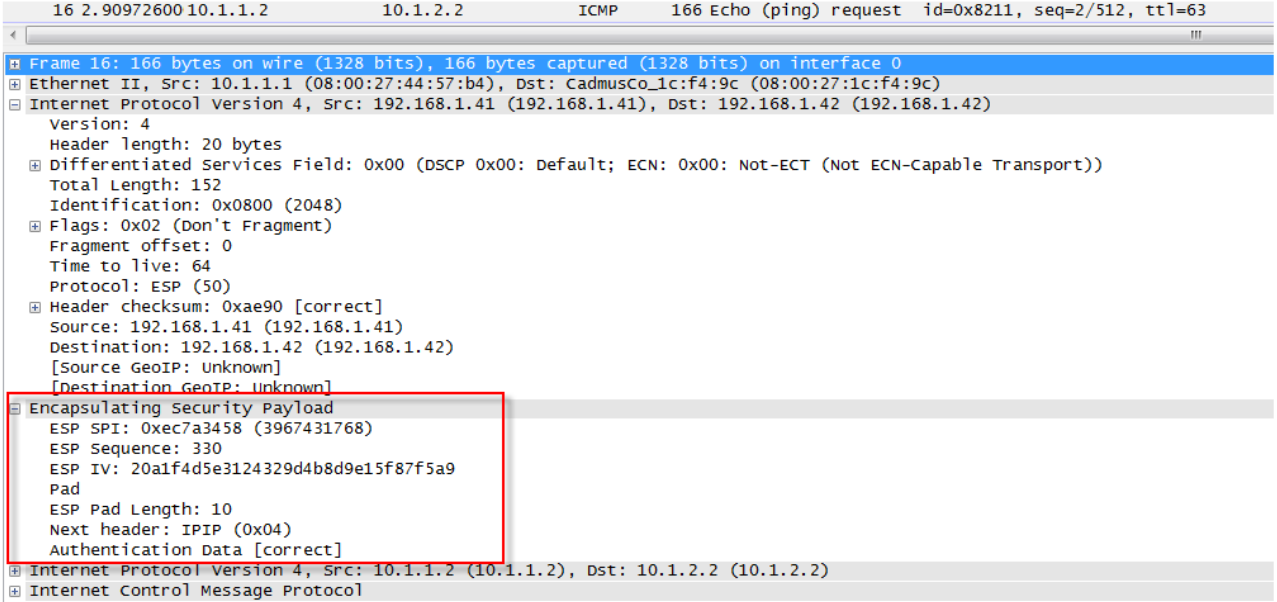
\includegraphics[width=11cm]{Imagenes/desencriptacionICMP.png}
		\caption{Tr\'afico desencriptado}\label{img030}
	\end{figure}	
	\begin{figure}[H]
		\centering
		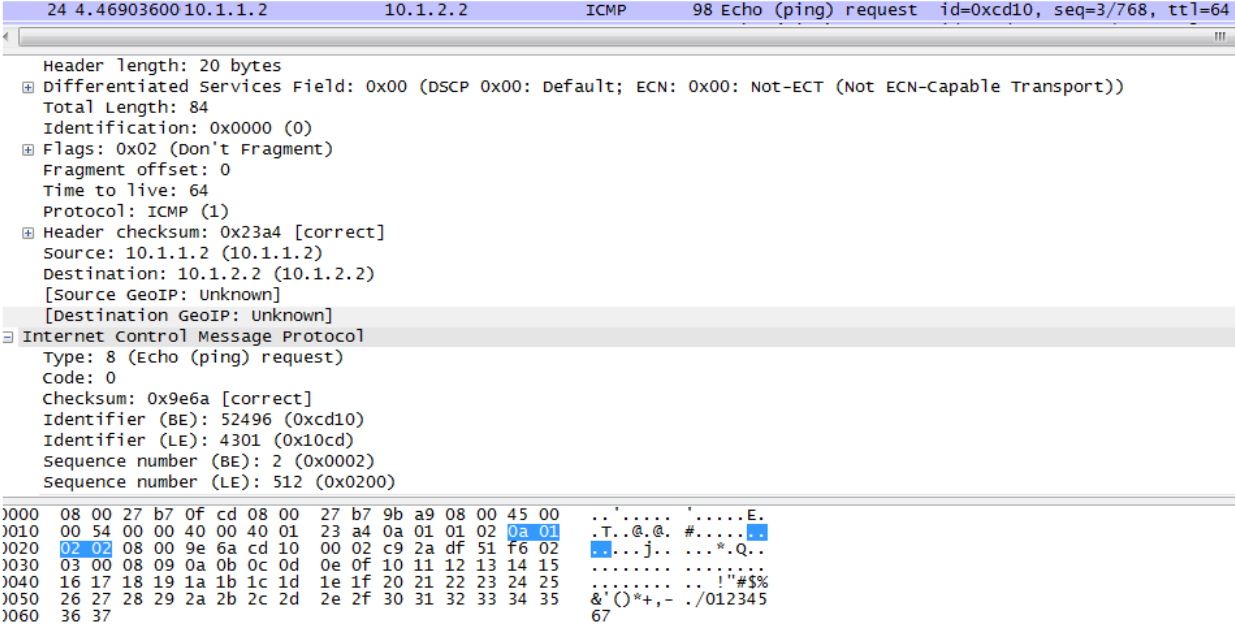
\includegraphics[width=11cm]{Imagenes/PingNoDesencriptado.png}
		\caption{Tr\'afico encriptado nuevamente por tener claves erroneas}\label{img031}
	\end{figure}	
		
		
	\newpage
	\section{Conclusiones}
	
	\indent Se comprobó que si un túnel IPSec en modo ESP es configurado correctamente entre dos redes privadas, estableciendo una VPN, es imposible sin conocer las claves de las SA’s determinar el tráfico que se intercambia
a través de ella. Por otro lado al usar el método de protección de identidad, además de impedir que personas ajenas a la comunicación puedan ver los paquetes, también se evita que tengan información acerca de quienes están intercambiando tráfico.
	


	
		
\end{document}

